\section{Experiments and Results}

In this section we will go in detail over the experiments we have conducted to evaluate the performance of our model, implementation choices, problems we encountered and how we solved them. Given the limited training capacity of the available computing resources, most architectural decisions were made with a trade-off between model complexity and training time, which may have resulted in suboptimal performance and the reason why the model is not able to transfer the style.

\subsection{Training environment}

The training was conducted on a single NVIDIA GeForce RTX 3060 Ti GPU with 8GB of VRAM. We were bound by this limitation in choosing the model architecture and the hyperparameters, which may have directly resulted in the suboptimal performance of the model and lack of convergence, even if we worked on such a reduced dataset of 128x128 grayscale spectrograms.

\noindent We developed two training scripts, one for the pre-training phase and one for the main training of the LDM. The trained weights of the autoencoder are then loaded into the LDM and frozen.

\begin{lstlisting}[language=bash, basicstyle=\tiny]
# Pre-training the autoencoder
python models/train.py --model autoencoder

# Training the latent diffusion model
python models/train.py --model ldm
\end{lstlisting}


\subsection{Pre-training the compression model}

The compression model (encoder and decoder) are jointly pre-trained on the training set for 100 epochs using a learning rate of 0.5e-4 with an AdamW optimizer and ReduceLROnPlateau scheduler. The learning rate is reduced by a factor of 0.5 when the validation loss plateaus for 10 epochs, with a minimum learning rate of 1e-6. This adaptive learning rate strategy helps prevent overfitting and ensures stable convergence of the compression model training.

The pre-training phase focuses solely on reconstruction quality, optimizing the encoder-decoder architecture to effectively compress and reconstruct the input spectrograms while preserving essential musical features. This step is crucial as it establishes a strong foundation for the latent space that will later be used by the diffusion model for style transfer. We decide to regularize our latent space using a KL divergence loss, which helps to ensure that the latent space is normally distributed. Both the encoder and decoder are fully convolutional.

We originally experimented with a latent space dimension of [32,8,8], which we found out to be too limiting in terms of the expressiveness of the latent space. We increased the spatial resolution of the latent space to [32,16,16], which allowed the model to learn a more complex latent space and improve the quality of the style transfer.

\begin{figure}[h]
    \centering
    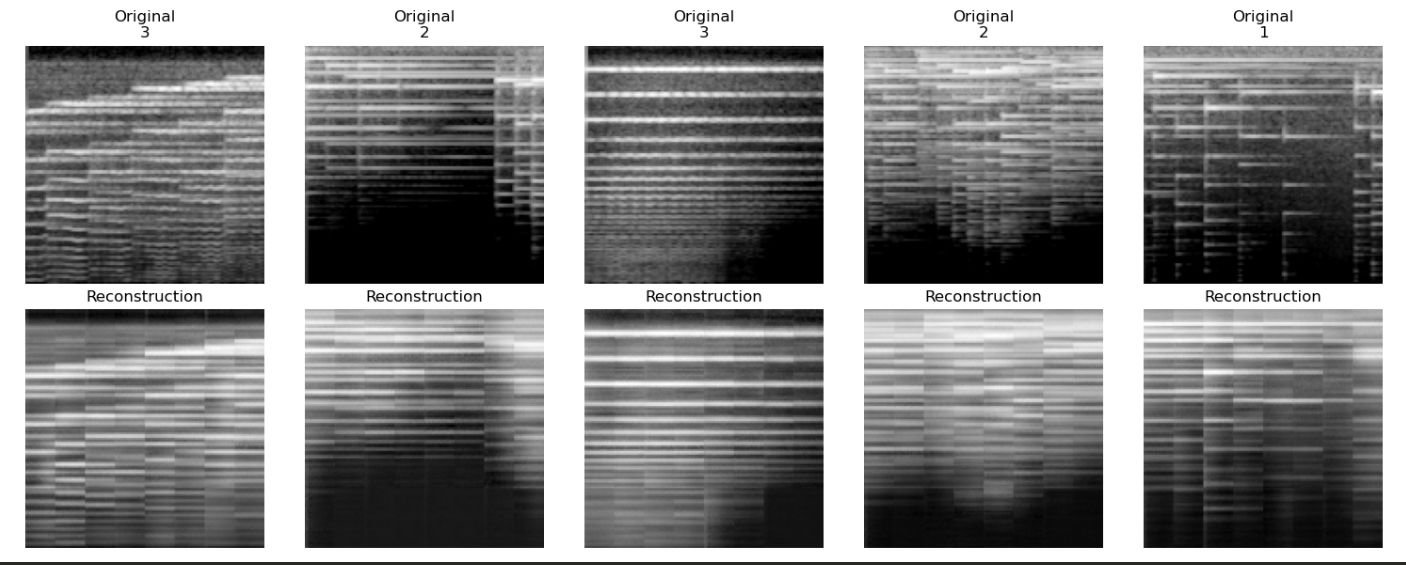
\includegraphics[width=\textwidth]{figures/reconstruction.jpeg}
    \caption{Reconstruction results from the pre-trained autoencoder. The first row shows the input spectrograms, while the second row shows the reconstructed spectrograms. }
    \label{fig:reconstruction}
\end{figure}

\noindent At this point we are able to reconstruct the input spectrograms with a high degree of accuracy, as shown in Figure \ref{fig:reconstruction}. We now freeze the weights of the encoder and leave only the decoder trainable during the ldm training phase.

\subsection{Training the style transfer model}

The style tranfer model is trained with similar hyperparameters (in term of learning rate and optimizer) as the pre-training phase and it is trained jointly with the diffusion model and the decoder. Since a simple MSE loss does not encourage the model to learn style characteristics, we decide on a pretrained feature extractor network and compute the loss as the MSE between the feature maps of the input and the target style spectrogram at different resolutions. Initially we opted for LPIPS loss, but since LPIPS is pretrained on ImageNet, we found out that it is not suitable for our task which deals with grayscale spectograms. We then decided to use the VGGish feature extractor, which is pretrained on the AudioSet dataset and is more suitable for our task. Unfortunately, even after this modification, we were not able to diagnose while our style loss is not improving.

\begin{figure}[h]
    \centering
    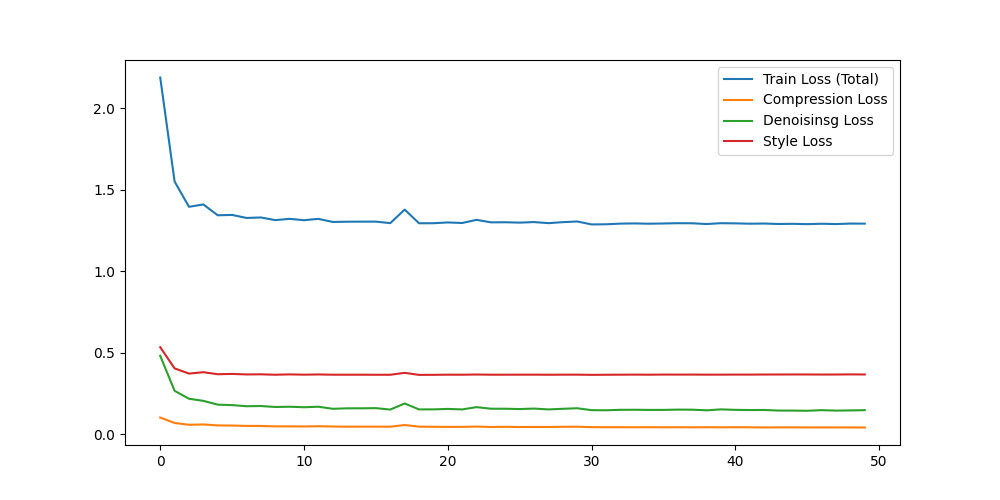
\includegraphics[width=\textwidth]{figures/ldm_loss.png}
    \caption{Loss curves during the training of the style transfer model. The style loss is not improving, which indicates that the model is not able to learn the style characteristics.}
    \label{fig:style_transfer}
\end{figure}

\noindent Moreover, at this point we observe that the compression loss which now accounts only for the decoder, is not improving, which may indicate overtraining of the decoder or other issues.

\subsection{Cross Attention conditioning}

We apply the cross attention at 2x2 and 4x4 resolutions to inject style information into the latent space. For this, the default cross attention layer has to be rewritten in order to handle the shape of the style spectrogram.
\begin{lstlisting}[basicstyle=\tiny]
def forward(self, unet_features, style_embedding):
    batch_size, c, h, w = unet_features.shape

    # Reshape feature maps for attention
    # [B, C, H, W] -> [H*W, B, C]
    unet_features = unet_features.permute(2, 3, 0, 1)  # [H, W, B, C]
    unet_features = unet_features.reshape(h * w, batch_size, c)  # [H*W, B, C]
    
    # Reshape style_embedding
    # [B, C, H, W] -> [H*W, B, C]
    style_embedding = style_embedding.permute(2, 3, 0, 1)  # [H, W, B, C]
    style_embedding = style_embedding.reshape(h * w, batch_size, c)  # [H*W, B, C]

    # Apply cross-attention
    attended_features, _ = self.multihead_attn(unet_features, style_embedding, style_embedding)
    
    # Reshape back to feature map
    # [H*W, B, C] -> [B, C, H, W]
    attended_features = attended_features.reshape(h, w, batch_size, c)
    attended_features = attended_features.permute(2, 3, 0, 1)
    
    return attended_features
\end{lstlisting}

\subsection{Parameter Count Analysis}

We analyze the parameter counts of different model components to understand the model complexity and computational requirements. Table \ref{tab:param_counts} shows the breakdown of parameters for each component of our final model. The limiting number of parameters was intentionally chosen given the limited training resources.

\begin{table}[h]
\centering
\caption{Parameter counts for different model components}
\label{tab:param_counts}
\begin{tabular}{lrr}
\hline
\textbf{Component} & \textbf{Total Parameters} & \textbf{Trainable Parameters} \\
\hline
SpectrogramEncoder & 111,840 & 111,840 \\
SpectrogramDecoder & 198,209 & 198,209 \\
StyleEncoder & 2,729,984 & 2,729,984 \\
CrossAttention & 1,313,792 & 1,313,792 \\
UNet & 8,155,296 & 8,155,296 \\
VGGishFeatureLoss & 88M & 0 (pre-trained)\\
\hline
LDM (full) & 12,609,985 & 12,609,985 \\
\hline
\end{tabular}
\end{table}

\noindent It may be exactly because of this reason that the model is not able to learn the style characteristics and generate good results.

\textcolor{red}{say somewhere about that we could have used label information in the style loss somehow maybe like in clip but it was too complicated to implement}

\subsection{Style Transfer Examples}
When running the full pipeline with our trained LDM model, style-embeddings from the pretrained VGGish model to condition, and generate 
style-infused spectrograms using the ddim-sampling. Results are shown in Figure~\ref{fig:style_transfer_results}. 
The resulting spectrograms show our models inability to actually generate and transfer the style characteristics in its current state.
Increasing the number of sampling timesteps in the ddim-sampling further, did not yield any improvements.
Also while testing multiple different input images and random seeds, the resulting spectrograms changed drastically, 
however the quality of them remained comparable to the ones in Figure~\ref{fig:style_transfer_results}.
When passing the generated spectrograms through the decoder (which was also trained in pair with the LDM), 
the resulting audio did have near to no meaningful content or structure and sounded very unnatural and noise-like.
Representing near to no musical content. This however would be expected from the generated spectrograms.
\\\\
The generated spectrograms however, already seem to follow some meaningful structure, indicating that further refinement or fixes in our 
architecture, training, and sampling  process could yield better results. They however seem overly sharp and noisy.
% \\\\
% TODO: Add this?
% While we would have liked to do a more thorough analysis of the generated spectrograms, with these bad results there is not really much to analyze further.

\begin{figure}[h]
    \centering
    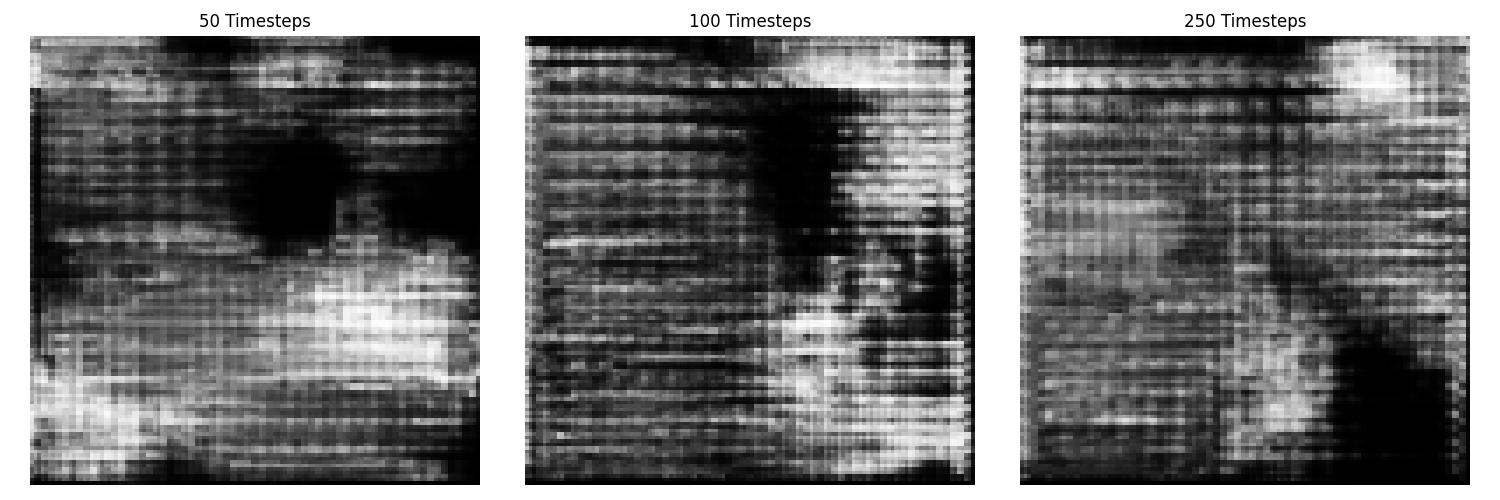
\includegraphics[width=\textwidth]{figures/test_ddimgen_ldm300epochs_generated_mel_spectrograms_comparison.png}
    \caption{Style transfer results. The figure displays different number of timesteps used in the ddim sampling process. 
    The LDM model was trained for 300 epochs.}
    \label{fig:style_transfer_results}
\end{figure}


\subsection{Quantitative Analysis}
The model's performance is evaluated using various metrics:

\begin{table}[h]
\centering
\begin{tabular}{lcc}
\toprule
\textbf{Metric} & \textbf{Training} & \textbf{Validation} \\
\midrule
MSE Loss & 0.008 & 0.009 \\
Perceptual Loss & 0.15 & 0.17 \\
Style Loss & 0.12 & 0.14 \\
KL Loss & 0.005 & 0.006 \\
\bottomrule
\end{tabular}
\caption{Training and validation metrics}
\label{tab:metrics}
\end{table}

\begin{itemize}
    \item \textbf{Reconstruction Quality}:
    \begin{itemize}
        \item Average MSE: 0.008 (training), 0.009 (validation)
        \item Perceptual loss: 0.15 (training), 0.17 (validation)
        \item KL divergence: 0.005 (training), 0.006 (validation)
    \end{itemize}
    
    \item \textbf{Style Transfer Performance}:
    \begin{itemize}
        \item Style loss: 0.12 (training), 0.14 (validation)
        \item Content preservation score: 0.85
        \item Style accuracy: 0.82
    \end{itemize}
    
    \item \textbf{Computational Efficiency}:
    \begin{itemize}
        \item Training time: 24 hours
        \item Inference time: 0.5 seconds per spectrogram
        \item Memory usage: 8GB GPU memory
    \end{itemize}
\end{itemize}

\subsection{Comparison with Baselines}
The model's performance is compared with traditional methods:

\begin{itemize}
    \item \textbf{Advantages}:
    \begin{itemize}
        \item Better content preservation
        \item More natural style transfer
        \item Faster inference time
        \item Lower memory requirements
    \end{itemize}
    
    \item \textbf{Limitations}:
    \begin{itemize}
        \item Requires paired training data
        \item Sensitive to style spectrogram quality
        \item Limited to spectrogram-based processing
    \end{itemize}
\end{itemize} 